\section{Heaps}\label{sec:heaps}

\subsection{Motivation}

Heaps are a way storing ordered data so that both querying and insertion of data can be fast. In particular they allow us to implement the Priority Queue ADT.

Let us briefly discuss the priority queue ADT. The data for this ADT is a collection of items (often labelled ``PQ" for reasons that the reader may guess) where each item has an associated \textit{priority} (an element from a totally ordered set, often the integers). A priority queue has three operations: \texttt{insert(PQ, x, priority)}, \texttt{FindMax(PQ)}, \texttt{ExtractMax(PQ)}. As you might guess \ttt{insert} adds $x$ into $PQ$ with the associated priority. \ttt{FindMax} returns the item with the highest priority. If there are multiple items with the highest priority then any one of them can be returned (the ADT does not specify which one). \ttt{ExtractMax} returns the item with the highest priority and removes it from $PQ$.

There are several ways we can try and implement this ADT. A rather naive way would be to use a linked list. Insertion adds an element to the head of list, making it $\Theta(1)$, which seems promising, but in order to find/extract the max we would have to iterate over every element in the list making both of those operations $\Theta(n)$. Things are slightly better if we order the list since this makes finding and extracting the maximum $\Theta(1)$ but now insertion is $\Theta(n)$ in the worst case (for example, if the item being added being added is bigger/smaller than all the items in the list then we need to iterate over every element of the list, depending on how the list is ordered). 
Another alternative is to use a Binary tree. In this case, all the operations are $\Theta(n)$ in the absolute worst case if the tree is unbalanced (effectively becoming a linked list) since finding the maximum requires us to to iterate all the way down. However if the tree is balanced the operations would $\Theta(\log n)$. Of course balancing a tree or keeping it balanced incurs its own cost. This is what inspires heaps: sort the data a bit so that querying of data is easy but not too sorted so that the structure can be maintained efficiently.

\subsection{Implementation}
We first need to talk about what a \textit{nearly complete binary tree} is. This is a binary tree where every row is completely filled, except possibly the last one (if the last is filled then it would be a \textit{complete} binary tree) and the last row we begin filling in from the left. Note this means that for every $N \in \N$, there is a unique configuration of $N$ nodes making a nearly complete binary tree (this is an important property which we use many times).

A heap, then, is nearly complete binary tree that satisfies the heap property. For a \textit{maxheap}, the heap property is that every node is greater than or equal to its immediate children (which, by recursion, implies that the root is the largest node). As one can guess, for a \textit{minheap}, the heap property is when every node is less than or equal to its immediate children.

\begin{figure}[h]
    \centering
    \begin{subfigure}[b]{0.4\textwidth}
        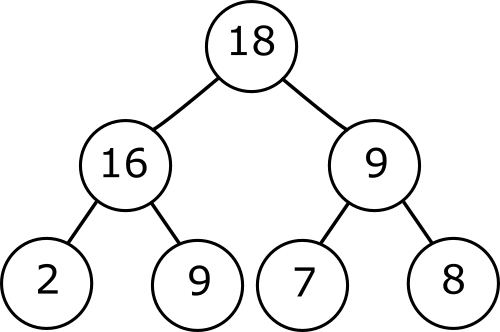
\includegraphics[scale = 0.3]{Images/heap_example.png}
        \caption{Heap Example}
        \label{fig:rsource}
    \end{subfigure}
    ~
    \begin{subfigure}[b]{0.4\textwidth}
        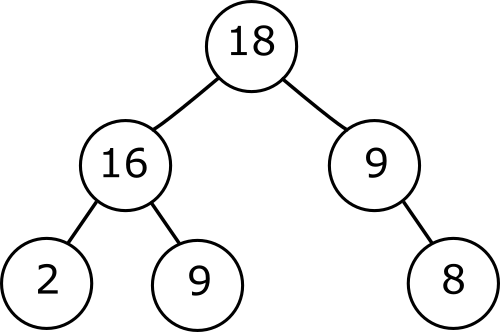
\includegraphics[scale=0.3]{Images/heap_non_example.png}
        \caption{Heap Non-example}
        \label{fig:lsource}
    \end{subfigure}
\end{figure}

The question then becomes how do the different operations work with this structure. The easiest, of course, is \texttt{FindMax} where it only needs return the root of the tree. The other two are a bit more tricky. The general principle when modifying heaps is that we first maintain its shape as a nearly complete binary tree and then modify the values within so that they satisfy the heap property.

Let us first begin with insertion. Given any tree, we know exactly where an additional node should go since every heap of $N$ items has a unique configuration. After a node is added and the value place inside, we compare this added node to its parent to verify whether the heap property is satisfied. If it is, then we are done. If not, we swap the parent and child and ask again whether the newly modified parent (which will contain the inserted value) satisfies the heap property or not. If not, we swap it with its parent again. We continue doing this until the heap property is satisfied or the inserted value reaches the top of the tree. This process is known as ``bubbling up'' or ``max heapifying''. This can occur at most as many times as the height of the tree, so this operation is $\Theta(\log n)$ in the worst case.

\begin{figure}[h]
    \centering
    \begin{subfigure}[b]{0.3\textwidth}
        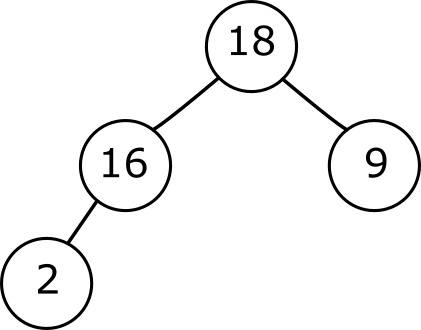
\includegraphics[scale = 0.3]{Images/insertion_step0.png}
        \caption{Starting heap to which we will add 17}
        \label{fig:insert_step0}
    \end{subfigure}
    ~
    \begin{subfigure}[b]{0.3\textwidth}
        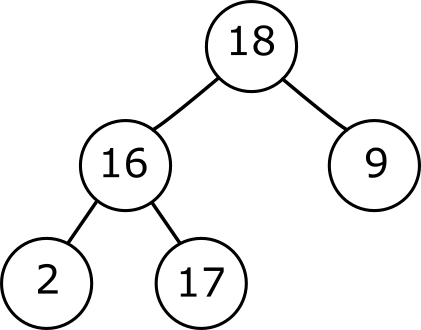
\includegraphics[scale=0.3]{Images/insertion_step1.png}
        \caption{Step1: Add node to maintain heap structure}
        \label{fig:insert_step1}
    \end{subfigure}
    ~
    \begin{subfigure}[b]{0.3\textwidth}
        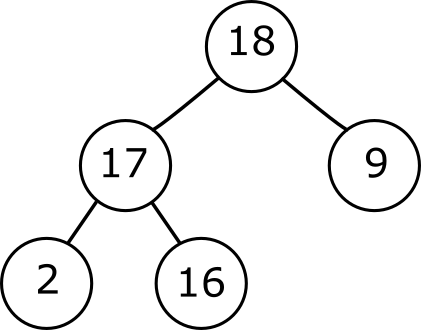
\includegraphics[scale=0.3]{Images/insertion_step2.png}
        \caption{Step 2: Swap 17 and 16 to satisfy the max heap property}
        \label{fig:insert_step2}
    \end{subfigure}
\end{figure}

Extraction of max is a bit more tricky. After we return the maximum value, we remove the very last item of the heap (recall there is only one possible configuartion for any number of nodes, so we know that the last node needs to be removed anyway) and place it as the root. In this case, the heap property is almost certainly not satisfied (although if it is, we are done!). If we need to, we then swap the root with the larger of its children and continue this process of ``bubbling down'' until the heap property is satisfied. Once again this process is $\Theta(\log n)$ in the worst case.

% TODO: Add figure for extract max

\subsection{Array Implementation}
The wonderful thing about heaps is that they can be stored as arrays. This is because, as we've said multiple times, there is unique configuration of a heap for any number of nodes, hence given a list of numbers, we know exactly what heap it would correspond to. The benefit of storing this data as an array is that it becomes very easy to access the children or parent of a node: if a node is at index $i$, its left child will be at index $2i$, its right child is at index $2i + 1$ and the parent is $\lfloor \frac{i}{2} \rfloor$ (Note: this assumes we start indexing from 1 \textit{not} from 0).

\begin{figure}[h]
    \centering
    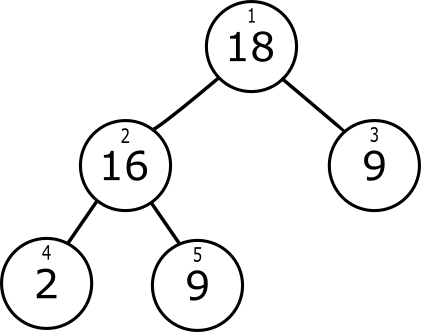
\includegraphics[scale=0.45]{Images/heap_array_tree.png}
    \caption{Heap Example in a tree}
    \label{fig:heap_tree}
\end{figure}
\begin{figure}[h]
    \centering
    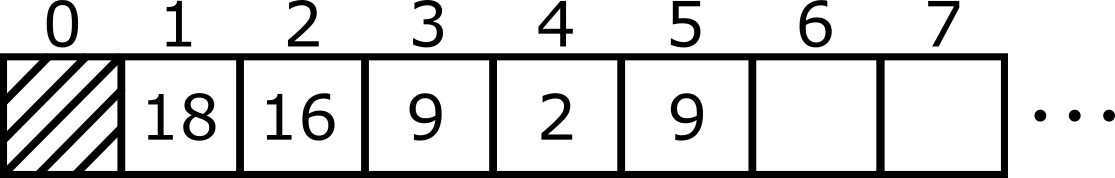
\includegraphics[scale=0.45]{Images/heap_array.png}
    \caption{Same heap in an array}
    \label{fig:heap_array}
\end{figure}

\section{Heapsort}\label{sec:heapsort}
As mentioned heaps are partially sorted. One might wonder how much effort it would take to get it completely sorted, i.e. turn it into a sorted list. We recall that the largest element of the heap is always at the root. So by repeatedly calling \texttt{ExtractMax} on a heap, we should be able to get a sorted list. Remembering that heaps are almost always implemented as arrays, we might get another brilliant insight: do the sorting in place.

For example, we first swap the first and last element in the heap, do the bubbling down and then decrement the heapsize. By decrementing the heapsize, the root which was at the end of the heap is moved out of it. This means that it's already in the position it should be! (assuming we are sorting the list in non-decreasing order).

\begin{figure}[h]
    \centering
    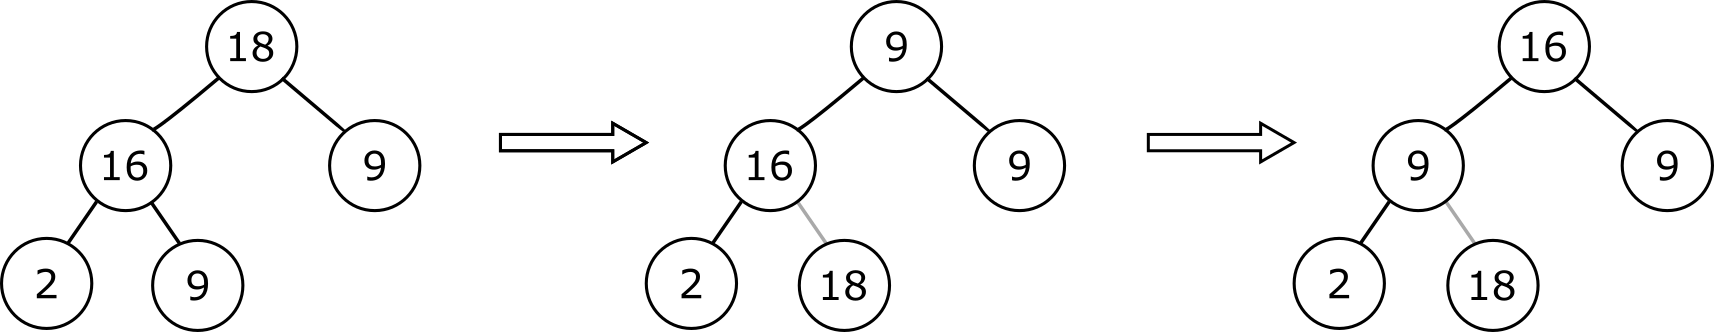
\includegraphics[scale=0.3]{Images/heap_sort_tree.png}
    \caption{Extract max in a tree}
    \label{fig:heap_sort_tree}
\end{figure}

\begin{figure}[h]
    \centering
    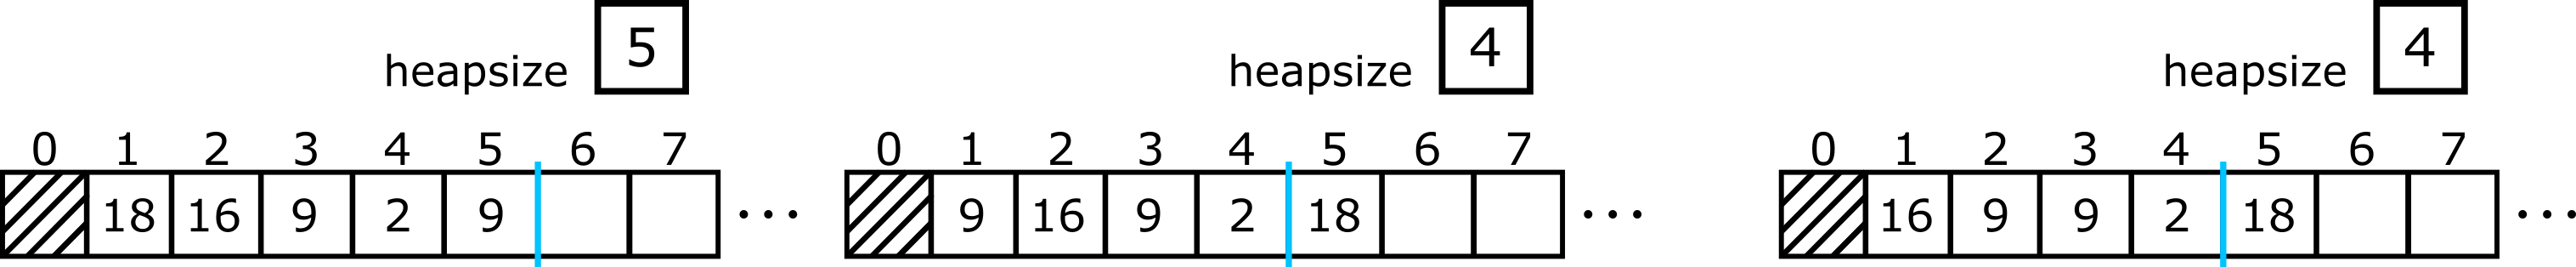
\includegraphics[scale=0.3]{Images/heap_sort_array.png}
    \caption{Extract max in array (note placement of 18). Grey edge indicates removed edge.}
    \label{fig:heap_sort_array}
\end{figure}

As the 18 is past heapsize, we need not worry about it anymore (from the perspective of the heap, it is no longer in it). It is easy to see that as we continue this we will continue placing the largest elements at the end, thereby getting a non-decreasing list at the end.

Let's see what the bubbling-down, also known as MaxHeapify, would look like in code.

\begin{lstlisting}
def maxHeapify(L, i):
    l = left(i) # if 1-based indexing left(i) = 2i
    r = right(i) # if 1-based indexing right(i) = 2i + 1
    if l <= L.heapsize and L[l] > L[i]:
        largest = l # stores index of the largest number
    else:
        largest = i
        
    if r <= L.heapsize and L[r] > L[largest]:
        largest = r
        
    if largest != i:
        exchange L[i] with L[largest]
        maxHeapify(L, largest)
\end{lstlisting}
\vskip.5em

Of course we don't quite have a sorting algorithm yet. We first need to see how to turn an unsorted list into a heap (starting with a heap means if you've already most of the work!).

The most obvious way of turning an unsorted list into a heap would be to start with an empty heap and repeatedly call \texttt{Insert} on the items of the sorted list to add them to the heap. Since \texttt{Insert} preserves the heap property, after all the items have been inserted, we will have a valid heap. Unfortunately, as is so often the case with computer science (and quite frankly life) the most obvious solution is often not very good.

It is easy to see that in the worst case, this algorithm is $O(n \log n)$ since each insert takes at most $\log n$ time and we do $n$ insertions. With a bit more though we can also conclude that this algorithm is also $\Omega(n \log n)$. Recall from above that this requires us to find a family of inputs where the runtime \textit{is} actually $n \log n$. Suppose we apply this algorithm on an increasing list. Then every insertion will take $\log h$ time where $h$ is the height of the tree when the particular insert is called. Note that in any nearly complete binary tree, at least half of the nodes are leaves (induction might be the simplest way of convincing oneself of this fact). These leaves are at a depth of $\log n$ or $\log n - 1$ (if the tree is a complete binary tree then all leaves are at depth $\log n$, otherwise there are some leaves at depth $\log n - 1$). For each of those $\lceil \frac{n}{2} \rceil$ leaves, at least $\log n - 1$ swaps are done. Thus the algorithm is in $\Omega(\lceil \frac{n}{2} \rceil \log(n) - 1)$ which, via asymptotic notation, means that the algorithm is $\Omega(n \log n)$.

Let's see if we can do any better. The problem with the above algorithm is that the most expensive operation is at the leaves which are also the most common node in a heap. Ideally what we would want is an algorithm that is cheap for leaves and maybe a bit more expensive for other nodes. 

One might remember that heaps are recursive in nature. That is, in a heap the left and right child of any node are themselves heaps. Leaves can then be thought of one-node heaps. Inspired by this, and by the previous discussion of \texttt{MaxHeapify}, we might consider the following: put the unsorted array into a nearly complete binary tree and work backwards by calling \texttt{MaxHeapify} on every node. Nodes that are near the bottom of the tree (which are the most frequent ones) have shorter subtrees therefore are cheaper to correct. Indeed this change allows the algorithm to be $O(n)$ rather than $O(n \log n)$.

Let us work this out mathematically. There are $\frac{n}{2}$ leaves (for now we assume $n$ to be a power of 2) hence they are trees of height 0. There are $\frac{n}{4}$ nodes which are rooted at trees of height 1 (these are of course the parents of all the leaves). We continue similarly to conclude that there are $\frac{n}{2^{k}}$ nodes which have trees of height $k - 1$ for $k$ between $1$ and $\log n$. Thus the total time of this algorithm is
\begin{align*}
    \sum_{h = 0}^{\lfloor \log n\rfloor} h \cdot \left\lceil \frac{n}{2^{h + 1}}  \right\rceil = O\left( \frac{n}{2} \sum_{h = 0}^{\lfloor \log n \rfloor} \frac{h}{2^h} \right)
    = O \left( n \right)
\end{align*}
where we use the fact that $\sum_{k = 1}^{\infty} kr^k = \frac{r}{(1 - r)^2}$ provided that $0 < r < 1$ (this is known as Gabriel's staircase series).